\documentclass[fleqn]{book}

\usepackage{polski}
\usepackage[utf8]{inputenc}
\usepackage{amsthm}
\usepackage{amssymb}
\usepackage{amsmath}
\usepackage{booktabs}
\usepackage{dsfont}
\usepackage{pgfplots}
\usepackage{fancyhdr}
\usepackage{bookmark}
\usepackage{makeidx}
\usepackage{multirow}
\usepackage{gensymb}
\makeindex

\pgfplotsset{compat=1.13}

\newcommand*\conj[1]{\bar{#1}}
\newcommand*\abs[1]{\left|#1\right|}

\newtheorem{definition}{Definicja}[section]
\newtheorem{theorem}{Twierdzenie}[section]

\pagestyle{fancy}
\lhead{Notatki - Matematyka}
\rhead{Adrian Startek}

\title{Notatki - Matematyka}
\author{Adrian Startek}
\date{Studia I stopnia}

\begin{document}
    \frontmatter
    \maketitle
    \tableofcontents
    \mainmatter
    \part{Semestr I}
    \chapter{Elementy logiki i teorii mnogości}
    \section{Podstawowe definicje i oznaczenia}
    \begin{definition}
        \index{zdanie logiczne}
        Zdanie logiczne: zdanie, któremu można przyporządkować wartość logiczną "prawda"(1) lub "fałsz"(0).
    \end{definition}
    \begin{definition}
        \index{tautologia}
        Tautologia: zdanie logiczne, które zawsze jest prawdziwe.
    \end{definition}
    \begin{definition}
        \index{funckcja!zdaniowa}
        Funkcja zdaniowa $\phi(x)$: wyrażenie, które po podstawieniu konkretnej wartości $x$ staje się zdaniem logicznym.
    \end{definition}
    \begin{definition}
        \index{para uporządkowana}
        Para uporządkowana (x,y): zbiór $\{\{x\},\{x,y\}\}$. Elementem pierwszym w parze jest ten, który jest elementem obu zbiorów, co jednoznacznie określa kolejność.
    \end{definition}

    \subsection{Zbiory liczbowe}
        $\mathbb{N}$ - zbiór liczb naturalnych\\
        $\mathbb{Z}$ - zbiór liczb całkowitych\\
        $\mathbb{Q}$ - zbiór liczb wymiernych\\
        $\mathbb{R}$ - zbiór liczb rzeczwistych

        \paragraph{} Fakt należenia elementu x do zbioru A oznacza się przez $x \in A$. Analogicznie, "x nie należy do zbioru A" ocznacza się $x \notin A$.
        \paragraph{} Zbiór można definiować podając jego elementy wprost: $A = \{a, b, c\}$ lub zadając warunek na przynależność elementów do zbioru: $A = \{x \in X: \phi (x)\}$. 

    \subsection{Kwantyfikatory}
        \paragraph{Kwantyfikator ogólny.} Wyrażenie "dla każdego x należącego do X zachodzi $\phi(x)$" oznacza się: $\forall_{x \in X} \, \phi(x)$
        \paragraph{Kwantyfikator szczególny.} Wyrażenie "istnieje x należący do X, dla którego zachodzi $\phi(x)$" oznacza się: $\exists_{x \in X} \, \phi(x)$
        \paragraph{Zaprzeczenia kwantyfikatorów.} Zachodzi:
        \begin{equation*}
            \neg [\,\forall_{x \in \mathbb{R}} \, \phi(x)\,] \Leftrightarrow \exists_{x \in \mathbb{R}} \, \neg \phi(x)
        \end{equation*}
        \begin{equation*}
            \neg [\,\exists_{x \in \mathbb{R}} \, \phi(x)\,] \Leftrightarrow \forall_{x \in \mathbb{R}} \, \neg \phi(x)
        \end{equation*}
        \begin{equation*}
            \neg [\,\forall_{x \in \mathbb{R}} \, \phi(x) \vee \psi(x)\,] \Leftrightarrow \exists_{x \in \mathbb{R}} \, \neg \phi(x) \wedge \neg \psi(x)
        \end{equation*}
        \begin{equation*}
            \neg [\,\exists_{x \in \mathbb{R}} \, \phi(x) \wedge \psi(x)\,] \Leftrightarrow \forall_{x \in \mathbb{R}} \, \neg \phi(x) \vee \neg \psi(x)
        \end{equation*}

\section{Rachunek zdań logicznych}
    \subsection{Ważniejsze operacje na zdaniach}
        \paragraph{Negacja}
        Wartością negacji zdania logicznego jest wartość odwrotna do wartości tego zdania (tabela \ref{tab:negacja}).
        \begin{table}[htbp!]
            \centering
            \caption{Negacja}
            \label{tab:negacja}
            \vspace{3mm}
            \begin{tabular}{cc}
                \textbf{$p$} & \textbf{$\neg p$} \\
                \midrule
                0 & 1\\
                1 & 0 \\
                \bottomrule
            \end{tabular}
        \end{table}

        \paragraph{Alternatywa}
        Alternatywa przyjmuje wartość "prawda", jeśli co najmniej jedno ze zdań jest prawdziwe (tabela \ref{tab:alternatywa}).
        \begin{table}[htbp!]
            \centering
            \caption{Alternatywa}
            \label{tab:alternatywa}
            \vspace{3mm}
            \begin{tabular}{ccc}
                \textbf{$p$} & \textbf{$q$} & \textbf{$p \vee q$} \\
                \midrule
                0 & 0 & 0\\
                0 & 1 & 1\\
                1 & 0 & 1\\
                1 & 1 & 1\\
                \bottomrule
            \end{tabular}
        \end{table}

        \paragraph{Koniunkcja}
        Koniunkcja przyjmuje wartość "prawda", tylko jeśli oba zdania są prawdziwe (tabela \ref{tab:koniunkcja}).
        \begin{table}[htbp!]
            \centering
            \caption{Koniunkcja}
            \label{tab:koniunkcja}
            \vspace{3mm}
            \begin{tabular}{ccc}
                \textbf{$p$} & \textbf{$q$} & \textbf{$p \wedge q$} \\
                \midrule
                0 & 0 & 0\\
                0 & 1 & 0\\
                1 & 0 & 0\\
                1 & 1 & 1\\
                \bottomrule
            \end{tabular}
        \end{table}

        \paragraph{Implikacja}
        Implikacja ($p \Longrightarrow q$) jest prawdziwa, jeśli zarówno poprzednik ($p$) jak i następnik ($q$) są prawdziwe lub \textbf{poprzednik jest fałszywy (z fałszu wynika wszystko)}. (tabela \ref{tab:implikacja})
        \begin{table}[htbp!]
            \centering
            \caption{Implikacja}
            \label{tab:implikacja}
            \vspace{3mm}
            \begin{tabular}{ccc}
                \textbf{$p$} & \textbf{$q$} & \textbf{$p \Longrightarrow q$} \\
                \midrule
                0 & 0 & 1\\
                0 & 1 & 1\\
                1 & 0 & 0\\
                1 & 1 & 1\\
                \bottomrule
            \end{tabular}
        \end{table}
        
        \paragraph{Równoważność}
        Równoważność przyjmuje wartość "prawda" jeśli oba zdania mają tą samą wartość (tabela \ref{tab:rownowaznosc}).
        \begin{table}[htbp!]
            \centering
            \caption{Równoważność}
            \label{tab:rownowaznosc}
            \vspace{3mm}
            \begin{tabular}{ccc}
                \textbf{$p$} & \textbf{$q$} & \textbf{$p \Leftrightarrow q$} \\
                \midrule
                0 & 0 & 1\\
                0 & 1 & 0\\
                1 & 0 & 0\\
                1 & 1 & 1\\
                \bottomrule
            \end{tabular}
        \end{table}
        
        \paragraph{Kreska Sheffera (NAND)}
        Zaprzeczenie koniunkcji (tabela \ref{tab:nand}).
        \begin{table}[htbp!]
            \centering
            \caption{NAND}
            \label{tab:nand}
            \vspace{3mm}
            \begin{tabular}{ccc}
                \textbf{$p$} & \textbf{$q$} & \textbf{$p \mid q$} \\
                \midrule
                0 & 0 & 1\\
                0 & 1 & 1\\
                1 & 0 & 1\\
                1 & 1 & 0\\
                \bottomrule
            \end{tabular}
        \end{table}
        
        \paragraph{NOR}
        Zaprzeczenie alternatywy (tabela \ref{tab:nor}). 
        \begin{table}[htbp!]
            \centering
                \caption{NOR}
                \label{tab:nor}
                \vspace{3mm}
                \begin{tabular}{ccc}
                    \textbf{$p$} & \textbf{$q$} & \textbf{$p\downarrow q$} \\
                    \midrule
                    0 & 0 & 1\\
                    0 & 1 & 0\\
                    1 & 0 & 0\\
                    1 & 1 & 0\\
                    \bottomrule
                \end{tabular}
        \end{table}
        
        \begin{theorem}
            Za pomocą \textbf{NAND} lub \textbf{NOR} można wyrazić wszystkie inne funktory.
        \end{theorem}
    
    \subsection{Ważniejsze tautologie}
        \begin{equation*}
            \tag{prawo tożsamości}
            p \Longrightarrow p
        \end{equation*}
        \begin{equation*}
            \tag{prawo symplifikacji}
            p \Longrightarrow (q \Longrightarrow p)
        \end{equation*}
        \begin{equation*}
            \tag{prawo podwójnej negacji}
            p \Leftrightarrow \neg(\neg p)
        \end{equation*}
        \begin{equation*}
            \tag{prawo wyłączonego środka}
            p \vee \neg p\end
        {equation*}
        \begin{equation*}
            (\neg p \Longrightarrow p) \Longrightarrow p
        \end{equation*}
        \begin{equation*}
            \tag{prawo Dunsa Szkota}
            \neg p \Longrightarrow (p \Longrightarrow q)
        \end{equation*}
        \begin{equation*}
            \tag{prawo De Morgana}
            \neg (p \vee q) \Leftrightarrow (\neg p) \wedge (\neg q)
        \end{equation*}
        \begin{equation*}
            \tag{prawo De Morgana}
            \neg (p \wedge q) \Leftrightarrow (\neg p) \vee (\neg q)
        \end{equation*}
        \begin{equation*}
            \neg(p \Longrightarrow q) \Leftrightarrow p \wedge (\neg q)
        \end{equation*}
        \begin{equation*}
            \neg(p \Leftrightarrow q) \Leftrightarrow (p \wedge \neg q) \vee (\neg p \wedge q)
        \end{equation*}

\section{Rachunek zbiorów}
    \subsection{Operacje i zależności}
        \paragraph{Zawieranie.} Zbiór A zawiera się w zbiorze B (A jest podzbiorem B), ozn. $A \subset B$, jeśli każdy element zbioru A jest również elementem zbioru B:
        \begin{equation*}
            A \subset B \Leftrightarrow \forall_{x\in A} \,  x\in B
        \end{equation*}
        
        \paragraph{Równość.} Zbiory A i B są równe, jeśli są one nawzajem swoimi podzbiorami:
        \begin{equation*}
            A = B \Leftrightarrow A \subset B \wedge B \subset A
        \end{equation*}

        \paragraph{Działania na zbiorach.} Definiuje się działania:
        \begin{equation}
            \tag{Suma zbiorów}
            A \cup B = \{\,x: x \in A \vee x \in B\,\}
        \end{equation}
        \begin{equation*}
            \tag{Iloczyn zbiorów}
            A \cap B = \{\,x: x \in A \wedge x \in B\,\}
        \end{equation*}
        \begin{equation*}
            \tag{Różnica zbiorów}
            A \setminus B = \{\,x: x \in A \wedge x \notin B\,\}
        \end{equation*}
        \begin{equation*}
            \tag{Iloczyn kartezjański}
            A \times B = \{\,(a,b): a \in A, b \in B\,\}
        \end{equation*}
        
        \paragraph{Dopełnienie zbioru.}
        \begin{definition}
            Dopełnieniem zbioru $A \subset C$ do zbioru C nazywa się zbiór wszystkich elementów należących do C, które nie należą do A:
            \begin{equation*}
                \setminus A = \{\,x \in C: x \notin A\,\}
            \end{equation*}
        \end{definition}

        \paragraph{Własności dopełnienia.}
        Niech $A \subset X$, $B \subset X$. Wtedy:
        \begin{equation*}
            \setminus(\,A \cup B\,) = (\,\setminus A\,) \cap (\,\setminus B\,)
        \end{equation*}
        \begin{equation*}
            \setminus(\,A \cap B\,) = (\,\setminus A\,) \cup (\,\setminus B\,)
        \end{equation*}
        \begin{equation*}
            \setminus(\,\setminus A\,) = A
        \end{equation*}

    \subsection{Relacje}
    \begin{definition}
        Relacją nazywa się dowolny podzbiór iloczynu kartezjańskiego skończonej liczby zbiorów.
    \end{definition}

Niech R będzie relacją zadaną na $X \times X$ (tj. R jest relacją dwuargumentową, która przyjmuje za argumenty elementy X). Dodatkowo, niech $xRy$ oznacza wyrażenie "pomiędzy x a y zachodzi relacja R". Wtedy:
\paragraph{R jest relacją zwrotną} $\Leftrightarrow \forall_{x \in X} \, xRx$
\paragraph{R jest relacją przeciwzwrotną} $\Leftrightarrow \forall_{x \in X} \, \neg (\,xRx\,)$
\paragraph{R jest relacją symetryczną} $\Leftrightarrow \forall_{x,y \in X} \, (\,xRy \Longrightarrow yRx\,)$
\paragraph{R jest relacją słabo antysymetryczną} $\Leftrightarrow \forall_{x,y \in X} \, (\,xRy \wedge yRx \Longrightarrow x = y\,)$
\paragraph{R jest relacją antysymetryczną} $\Leftrightarrow \forall_{x,y \in X} \, (\,xRy \Longrightarrow \neg(\,yRx\,)\,)$
\paragraph{R jest relacją przechodnią} $\Leftrightarrow \forall_{x,y,z \in X} \, (\,xRy \wedge yRz \Longrightarrow xRz\,)$
\paragraph{R jest relacją spójną} $\Leftrightarrow \forall_{x,y \in X} \, (\,xRy \vee yRx \vee y = x\,)$

    \chapter{Algebra liniowa}
    \section{Działanie, grupa, ciało}
\begin{definition}
    Niech G będzie dowolnym zbiorem. \textbf{Działaniem} (dwuargumentowym) w zbiorze G nazywamy dowolne odwzorowanie $f: G \times G \rightarrow G$.
\end{definition}

\begin{definition}
    Zbiór G z określonym działaniem $\circ$ - parę $(\,G, \circ\,)$ nazwiemy grupą, jeśli spełnione są następujące warunki:
    \begin{enumerate}
        \item Działanie $\circ$ jest łączne: 
            \begin{equation*}
                \forall_{a,b,c \in G} \, [\,(\,a \circ b\,) \circ c = a \circ (\,b \circ c\,)\,]
            \end{equation*}
        \item Istnieje element neutralny e:
            \begin{equation*}
                \exists_{e \in G} \, \forall_{a \in G} \, (\,a \circ e = e \circ a = a\,)
            \end{equation*}
        \item Dla każdego elementu a istnieje element odwrotny $a^{-1}$:
            \begin{equation*}
                \forall_{a \in G} \, \exists_{a^{-1} \in G} \, (\,a \circ a^{-1} = a^{-1} \circ a = e\,)
            \end{equation*}
    \end{enumerate}
    Jeżeli działanie $\circ$ jest dodatkowo przemienne, to $(\, G, \circ\,)$ nazwiemy \textbf{grupą przemienną} lub \textbf{Abelową} (Niels Henrik Abel - matematyk norweski). Opuszczając natomiast warunek 3 (istnienie elementu odwrotnego) otrzymamy definicję struktury ogólniejszej, zwanej \textbf{półgrupą}. 
\end{definition}

\begin{theorem}
    Jeśli $(\,G, \circ \,)$ jest grupą, to isteniej dokładnie 1 element neutralny.
\end{theorem}

\begin{proof}
    Załóżmy, że $e, e' \in G$ są elementami neutralnymi. Wtedy:
    \begin{equation*}
        e = e \circ e' = e' \circ e = e'
    \end{equation*}
    Co prowadzi do sprzeczności.
\end{proof}

\begin{theorem}
    Jeśli g i h są elementami grupy spełniającymi $g \circ h = e$, to są one wzajemnie odwrotne.
\end{theorem}

\begin{theorem}
    Jeśli $(\, G, \circ\, )$ jest grupą oraz $a \in G$ to istnieje dokładnie jeden element odwrotny $a^{-1}$.
\end{theorem}

\begin{definition}
    Zbiór G z określonymi działaniami "mnożenia" $\odot$ i "dodawania" $\oplus$ - trójkę $(\, G, \odot, \oplus\,)$ - nazywamy ciałem, jeżeli spełnione są warunki:
    \begin{enumerate}
        \item Oba działania są przemienne:
            \begin{equation*}
                \forall_{a,b \in G} \, (\,a \oplus b = b \oplus a\,)
            \end{equation*}
            \begin{equation*}
                \forall_{a,b \in G} \, (\,a \odot b = b \odot a\,)
            \end{equation*}
        \item Oba działania są łączne:
            \begin{equation*}
                \forall_{a,b,c \in G} \, [\, (\,a \oplus b\,) \oplus c = a \oplus (\,b \oplus c\,)\,]
            \end{equation*}
            \begin{equation*}
                \forall_{a,b,c \in G} \, [\, (\,a \odot b\,) \odot c = a \odot (\,b \odot c\,)\,]
            \end{equation*}
        \item Istnieje element neutralny dodawania ("zero" $\mathds{O}$) oraz element neutralny mnożenia ("jeden" $\mathds{1}$)
        \item Dla każdego elementu zbioru G istnieje element odwrotny względem dodawania:
            \begin{equation*}
                \forall_{a \in G} \, (\, a \oplus a^{-1} = a^{-1} \oplus a = \mathds{O}\,)
            \end{equation*}
            Dla każdego elementu, poza elementem neutralnym dodawania, istnieje element odwrotny względem mnożenia:
            \begin{equation*}
                \forall_{a \in G, a \neq \mathds{O}} \, (\, a \odot a^{-1} = a^{-1} \odot a = \mathds{1}\,)
            \end{equation*}
        \item Zachodzi rozdzielność mnożenia względem dodawania:
            \begin{equation*}
                \forall_{a,b,c \in G} \, [\, a \odot (\, b \oplus c\,) = (\, a \odot b \,) \oplus (\, a \odot c\, )\,]
            \end{equation*}
        \item Elementy neutralne działań są od siebie różne:
            \begin{equation*}
                \mathds{O} \neq \mathds{1}
            \end{equation*}
    \end{enumerate}
\end{definition}
\subsection{Liczby zespolone}
\begin{definition}
    Niech $\mathds{C} := \mathds{R} \times \mathds{R}$. Określmy działania $\oplus ,\odot$:
    \begin{equation*}
        \oplus : (\,a,b\,)\oplus(\,c,d\,) = (\,a+c, b+d\,)
    \end{equation*}
    \begin{equation*}
        \odot : (\,a,b\,)\odot(\,c,d\,) = (\, ac-bd, ad+bc\,)
    \end{equation*}
    Trójkę $(\,G,\oplus,\odot\,)$ nazywamy ciałem liczb zespolonych.
\end{definition}

\paragraph{Postać kartezjańska.} Liczby zespolone posiadają naturalną interpretację geometryczną. Są one parami (uporządkowanymi) liczb rzeczywistych, więc można im przypisać punkty na płaszczyźnie. Liczbie $z = (\,a,b\,), z \in \mathds{C}$ odpowiada punkt o odciętej a i rzędnej b (rysunek \ref{fig:lba_zespolona}). Płaszczyznę, na której w ten sposób przedstawiamy liczby zespolone nazywamy \textbf{płaszczyzną Gaussa}.
\begin{figure}[htbp!]
    \centering
    \caption{Liczba zespolona jako punkt na płaszczyźnie}
    \label{fig:lba_zespolona}
    \vspace{3mm}
    \begin{tikzpicture}
        \begin{axis}[
                axis lines=middle,
                axis equal, 
                xmin=-4, 
                ymin=-4, 
                xmax=4, 
                ymax=4,
                xtick distance = 1,
                ytick distance = 1
            ]
            \addplot+ [black, nodes near coords, only marks, point meta=explicit symbolic] table [meta=label] {
                x   y   label
                2   3   z=(2,3)
            };
            \draw [dotted] (2,3) -- (2,0);
            \draw [dotted] (0,3) -- (2,3);
        \end{axis}
    \end{tikzpicture}
\end{figure}
\paragraph{Postać kanoniczna.} Podzbiór ciała $\mathds{C}$ złożony z liczb postaci $(\,x,0\,), x \in \mathds{R}$, również jest ciałem. Odwzorowanie $x \rightarrow (\,x,0\,)$ z $\mathds{R}$ w rozważany podzbiór $\mathds{C}$ zadaje izomorfizm ciał. Pozwala to na wprowadzenie utożsamienia $(\,x,0\,) \equiv x$. Wprowadźmy oznaczenie $i := (\,0,1\,)$ i nazwijmy ten element \textbf{jednostką urojoną}. Łatwo sprawdzić, że:
\begin{equation*}
    i^2 = (\,-1,0\,) \equiv -1
\end{equation*}
Dowolną liczbę zespoloną $z = (\,a,b\,)$ można przedstawić w postaci:
\begin{equation*}
    z = (\,a,b\,) = (\,a,0\,) + (\,b,0\,)(\,0,1\,) \equiv a+bi
\end{equation*}
Zapis liczby zespolonej z w postaci $z = a+bi$ nazywamy \textbf{postacią kanoniczną}. Liczbę $a \in \mathds{R}$ nazywamy \textbf{częścią rzeczywistą} liczby zespolonej i oznaczamy $\Re{z}$ (lub $Re(z)$). Analogicznie, liczbę $b \in \mathds{R}$ nazywamy \textbf{częścią urojoną} i oznaczamy $\Im{z}$ (lub $Im(z)$).
\begin{definition}
    \textbf{Liczbą sprzężoną} do liczby $z = a+bi$ nazywamy liczbę
    \begin{equation*}
        \conj{z} = a-bi
    \end{equation*}
\end{definition}
\begin{figure}[htbp!]
    \centering
    \caption{Interpretacja geometryczna liczby sprzężonej}
    \label{fig:lba_sprzezona}
    \vspace{3mm}
    \begin{tikzpicture}
        \begin{axis}[
                axis lines=middle,
                axis equal, 
                xmin=-4, 
                ymin=-4, 
                xmax=4, 
                ymax=4,
                xtick distance = 1,
                ytick distance = 1
            ]
            \addplot+ [black, nodes near coords, only marks, point meta=explicit symbolic] table [meta=label] {
                x   y   label
                2   3   $z=(2,3)$
                2   -3  $\conj{z}=(2,-3)$
            };
            \draw [dotted] (0,0) -- (2,3);
            \draw [dotted] (0,0) -- (2,-3);
        \end{axis}
    \end{tikzpicture}
\end{figure}
W interpretacji geometrycznej liczba sprzężona $\conj{z}$ jest odbiciem liczby $z$ względem osi odciętych (rysunek \ref{fig:lba_sprzezona}).
\paragraph{Postać trygonometryczna.} Niech $z = a+bi$ będzie liczbą zespoloną.
\begin{definition}
    \textbf{Modułem} liczby zespolonej $z$ nazywamy liczbę
    \begin{equation*}
        r = \mathopen|z\mathclose| = \sqrt{z\conj{z}} = \sqrt{a^2+b^2}
    \end{equation*}
\end{definition}
Moduł można interpretować jako długość odcinka pomiędzy początkiem układu współrzędnych a punktem reprezentującym liczbę zespoloną (rysunek \ref{fig:modul_lby_zespolonej}).
\begin{figure}[tbp!]
    \centering
    \caption{Moduł liczby zespolonej}
    \label{fig:modul_lby_zespolonej}
    \vspace{3mm}
    \begin{tikzpicture}
        \begin{axis}[
                axis lines=middle,
                axis equal, 
                xmin=-4, 
                ymin=-4, 
                xmax=4, 
                ymax=4,
                xtick = {0},
                ytick = {0},
                extra x ticks = {2},
                extra x tick labels = {a},
                extra y ticks = {3},
                extra y tick labels = {b}
            ]
            \addplot+ [black, nodes near coords, only marks, point meta=explicit symbolic] table [meta=label] {
                x   y   label
                2   3   $(a,b)$
            };
            \addplot [blue, domain=0:2] {1.5*x}
                node [pos=0.5, sloped, style={yshift=8pt}] {r}
            ;
            \draw [dotted] (0,3) -- (2,3);
            \draw [dotted] (2,0) -- (2,3);
        \end{axis}
    \end{tikzpicture}
\end{figure}
Niech $\varphi$ będzie kątem pomiędzy dodatnią półosią rzeczywistą a odcinkiem łączącym początek układu współrzędnych a punktem reprezentującym liczbę zezpoloną. Zachodzi wtedy:
\begin{equation*}
    r = \mathopen|z\mathclose|
\end{equation*}
\begin{equation*}
    sin \varphi = \frac{b}{\mathopen|z\mathclose|} \Longrightarrow b = \mathopen|z\mathclose| sin \varphi
\end{equation*}
\begin{equation*}
    cos \varphi = \frac{a}{\mathopen|z\mathclose|} \Longrightarrow a = \mathopen|z\mathclose| cos \varphi
\end{equation*}
Wynika z tego możliwość przedstawienia liczby zespolonej $z = a + bi$ w postaci:
\begin{equation*}
    z = a + bi = \mathopen|z\mathclose| cos \varphi + i \mathopen|z\mathclose| sin \varphi = \mathopen|z\mathclose|(cos \varphi + i\, sin \varphi)
\end{equation*}
\begin{theorem}
    Niech $z \in \mathds{C}$, $z = \mathopen|z\mathclose|(cos \varphi + i\, sin \varphi)$. Zachodzi:
    \begin{equation*}
        \forall_{n \in \mathds{N}} \, z^n = {\mathopen|z\mathclose|}^n (cos(n\varphi) + i\, sin(n\varphi))
    \end{equation*}
\end{theorem}
\begin{theorem}
    Niech $z \in \mathds{C}$, $z \neq (0,0)$, $z = \mathopen|z\mathclose|(cos\varphi + i\, sin\varphi)$.
    Istnieje dokładnie $n$ pierwiastków $n$-tego stopnia z liczby $z$. $k$-ty pierwiastek dany jest wzorem:
    \begin{equation*}
        w_k = \sqrt[n]{\mathopen|z\mathclose|}\left(cos\frac{\varphi+2k\pi}{n} + i\, sin \frac{\varphi+2k\pi}{n}\right), k \in \langle0; n-1 \rangle, k \in \mathds{N}
    \end{equation*}
    \begin{proof}
        Niech $w = \mathopen|w\mathclose|(cos \alpha + i\, sin \alpha)$ będzie pierwiastkiem $n$-tego stopnia z liczby $z$. Zatem:
        \begin{equation*}
            w^n = z
        \end{equation*}
        \begin{equation*}
            w^n = {\mathopen|w\mathclose|}^n(cos\, n\alpha + i\, sin\, n\alpha) = \mathopen|z\mathclose|(cos\varphi + i\, sin\varphi)
        \end{equation*}
        \begin{equation*}
            {\mathopen|w\mathclose|}^n = \mathopen|z\mathclose| \Longrightarrow \mathopen|w\mathclose| = \sqrt[n]{\mathopen|z\mathclose|}
        \end{equation*}
        \begin{equation*}
            n\alpha = \varphi+2k\pi \Longrightarrow \alpha = \frac{\varphi+2k\pi}{n}
        \end{equation*}
    \end{proof}
\end{theorem}
\section{Przestrzenie liniowe}
\begin{definition}
    Niech będzie dane ciało K oraz niepusty zbiór V z określonymi dwoma działaniami:
    \begin{equation*}
        \tag{dodawanie}
        \oplus: V \times V \ni (\,x,y\,) \rightarrow x \oplus y \in V
    \end{equation*}
    \begin{equation*}
        \tag{mnożenie przez element ciała}
        \odot: K \times V \ni (\,\lambda,x\,) \rightarrow \lambda \odot x \in V
    \end{equation*}
    Strukturę $(\,V,K,\oplus,\odot)$ nazwiemy \textbf{przestrzenią wektorową} (lub \textbf{liniową}) nad ciałem K, jeśli spełnione są warunki:
    \begin{enumerate}
        \item $(\,V,\oplus\,)$ jest grupą abelową
        \item $\forall_{x \in V}$:
            \begin{equation*}
                1\odot x = x
            \end{equation*}
        \item $\forall_{x \in V}\,\forall_{\alpha,\beta \in K}$:
            \begin{equation*}
                \tag{prawo łączności}
                \alpha\odot(\beta\odot x) = (\alpha\beta)\odot x
            \end{equation*}
        \item $\forall_{x,y \in V}\, \forall_{\alpha,\beta \in K}$:
            \begin{equation*}
                \tag{rozdzielność dodawania względem mnożenia}
                (\alpha + \beta)\odot x = \alpha \odot x \oplus \beta \odot x
            \end{equation*}
        \item $\forall_{x,y \in V}\, \forall_{\alpha \in K}$:
            \begin{equation*}
                \tag{rozdzielność mnożenia względem dodawania}
                \alpha\odot(x \oplus y) = \alpha\odot x \oplus \alpha\odot y
            \end{equation*}
    \end{enumerate}
    Elementy zbioru V nazywamy \textbf{wektorami}, a ciała K \textbf{skalarami}.
\end{definition}
\begin{theorem}
    Jeśli V jest przestrzenią liniową nad K, to dla każdego $v \in V, \, \alpha \in K$ zachodzi:
    \begin{enumerate}
        \item $ 0\odot v = \mathds{O}$
        \item $\alpha \odot \mathds{O} = \mathds{O}$
        \item $\alpha \odot v = \mathds{O} \Longrightarrow \alpha = 0 \vee v = \mathds{O}$
    \end{enumerate}
    \begin{proof} Kolejno:
        \begin{enumerate}
            \item
                \begin{equation*}
                    1\odot v = (1 + 0) \odot v = 1\odot v \oplus 0 \odot v
                \end{equation*}
                \begin{equation*}
                    1\odot v - 1\odot v = (1\odot v - 1\odot v) \oplus 0 \odot v
                \end{equation*}
                \begin{equation*}
                    \mathds{O} = 0 \odot v
                \end{equation*}
            \item
                \begin{equation*}
                    \alpha\odot\mathds{O} = \alpha(\mathds{O}\oplus\mathds{O}) = \alpha\odot\mathds{O}\oplus\alpha\odot\mathds{O}
                \end{equation*}
                \begin{equation*}
                    \alpha\odot\mathds{O}-\alpha\odot\mathds{O} = (\alpha\odot\mathds{O}-\alpha\odot\mathds{O})\oplus\alpha\odot\mathds{O}
                \end{equation*}
                \begin{equation*}
                    \mathds{O} = \alpha\odot\mathds{O}
                \end{equation*}
            \item
                \begin{equation*}
                    \alpha\odot v = \mathds{O}
                \end{equation*}
                Wystarczy pokazać, że jeśli  $\alpha\neq 0$, to $v = \mathds{O}$
                \begin{equation*}
                    \exists_{\alpha^{-1} \in K}\, \alpha\alpha^{-1} = 1
                \end{equation*}
                \begin{equation*}
                    \alpha\odot v = \mathds{O}
                \end{equation*}
                \begin{equation*}
                    \alpha\alpha^{-1}\odot v = \alpha^{-1}\odot\mathds{O}
                \end{equation*}
                \begin{equation*}
                    1\odot v = \mathds{O}
                \end{equation*}
                \begin{equation*}
                    v = \mathds{O}
                \end{equation*}
        \end{enumerate}
    \end{proof}
\end{theorem}
\begin{definition}
    Niech V będzie przestrzenią liniową nad ciałem K. Podzbiór $W \subset V$ nazywamy \textbf{podprzestrzenią liniową} przestrzeni V, jeśli W również jest przestrzenią liniową nad ciałem K.
\end{definition}
\begin{theorem}
    Podzbiór $W \subset V$ jest podprzestrzenią, wtedy i tylko wtedy, gdy zachodzi:
    \begin{equation*}
        \forall_{v_1,v_2 \in W} \, v_1 \oplus v_2 \in W
    \end{equation*}
    \begin{equation*}
        \forall_{\alpha \in K, v \in W} \, \alpha\odot v \in W
    \end{equation*}
\end{theorem}
\begin{theorem}
    \label{th:czesc_wspolna_podprzestrzeni}
    Niech V będzie przestrzenią liniową nad ciałem K, oraz niech $\{W_s\}$ będzie rodziną podprzestrzeni V. Wtedy:
    \begin{equation*}
        W = \bigcap_s W_s
    \end{equation*}
    jest podprzestrzenią liniową V.
        \begin{proof}
            Niech $v_1,v_2 \in W$
            \begin{equation*}
            v_1,v_2 \in W \Longrightarrow v_1,v_2 \in \bigcap_s W_s \Longrightarrow \forall_s v_1,v_2 \in W_s \Longrightarrow \forall_s v_1 \oplus v_2 \in W_s 
            \end{equation*}
            \begin{equation*}
                \Longrightarrow v_1\oplus v_2 \in \bigcap_s W_s \Leftrightarrow v_1\oplus v_2 \in W
            \end{equation*}
            Niech $v \in W, \alpha \in K$
            \begin{equation*}
                v \in W \Longrightarrow \forall_s v \in W_s \Longrightarrow \forall_s \alpha\odot v \in W_s \Longrightarrow \alpha\odot v \in W
            \end{equation*}
        \end{proof}
\end{theorem}
\begin{definition}
    Niech V będzie przestrzenią liniową nad ciałem K. Weźmy układ wektorów $\{v_1, \ldots, v_n\} \subset V$. Wektor
    \begin{equation*}
        v = \alpha_1 v_1 + \alpha_2 v_2 + \ldots + \alpha_n v_n
    \end{equation*}
    nazywamy \textbf{kombinacją liniową} wektorów $v_1,\ldots,v_n$.
\end{definition}
\begin{definition}
    \textbf{Powłoką liniową} podzbioru $M \subset V$ (gdzie V jest przestrzenią liniową) nazywamy zbiór wszystkich kombinacji liniowych wektorów z M i oznaczamy L(M).
\end{definition}
\begin{theorem}
    Niech V będzie przestrzenią liniową nad ciałem K i $M \subset V$ będzie podprzestrzenią. Powłoka liniowa L(M) jest podprzestrzenią liniową V.
    \begin{proof}
        \begin{equation*}
            v_1,v_2 \in L(M) \Longrightarrow
        \end{equation*}
        \begin{equation*}
            v_1 = \alpha_1 w_1 + \ldots + \alpha_n w_n, \, w_i \in M
        \end{equation*}
        \begin{equation*}
            v_2 = \beta_1 u_1 + \ldots + \beta_n u_n, \, u_i \in M
        \end{equation*}
        \begin{equation*}
            v_1 + v_2 = \alpha_1 w_1 + \ldots + \alpha_n w_n + \beta_1 u_1 \ldots \beta_n u_n 
        \end{equation*}
        zatem $v_1 + v_2$ jest kombinacją liniową wektorów $w_1,\ldots,w_n,u_1,\ldots,u_n \in M$, czyli $v_1 + v_2 \in M$.\\
        Niech $\alpha \in K, v \in L(M), v = \alpha_1 v_1+\ldots +\alpha_n v_n$
        \begin{equation*}
            \alpha v = \alpha(\alpha_1 v_1+\ldots +\alpha_n v_n) = \alpha\alpha_1 v_1+\ldots + \alpha\alpha_n v_n \in L(M)
        \end{equation*}
    \end{proof}
\end{theorem}
\begin{theorem}
    L(M) jest najmniejszą (w sensie zawierania zbiorów) podprzestrzenią V zawierającą M (jeżeli $W \subset V$ jest podprzestrzenią liniową V, taką że $M \subset W$, to $L(M) \subset W$).
    \begin{proof}
        Weźmy zbiór wszystkich podprzestrzeni liniowych zawierających M:
        \begin{equation*}
            \{W_s: s \in S\}
        \end{equation*}
        Niech
        \begin{equation*}
            \overline{W} = \bigcap_s W_s
        \end{equation*}
        Z twierdzenia \ref{th:czesc_wspolna_podprzestrzeni} $\overline{W}$ jest podprzestrzenią. Zauważmy: $\forall_s \overline{W} \subset W_s$. Pokażmy, że $\overline{W} = L(M)$, czyli $\overline{W} \subset L(M) \wedge L(M) \subset \overline{W}$. 
        \begin{enumerate}
            \item $\overline{W} \subset L(M)$. Skoro $\{W_s\}$ zawiera wszystkie podprzestrzenie zawierające M, to:
                \begin{equation*}
                    \exists_{s_0 \in S} W_{s_0} = L(M)
                \end{equation*}
            \item $L(M) \subset \overline{W}$. Niech $v \in L(M)$, wtedy:
                \begin{equation*}
                    v = \alpha_1 v_1 + \ldots + \alpha_n v_n, \, v_i \in M
                \end{equation*}
                \begin{equation*}
                    \forall_s \, \alpha_1 v_1 + \ldots +\alpha_n v_n \in W_s \Longrightarrow \forall_s \, \alpha_1 v_1 + \ldots +\alpha_n v_n \in \bigcap_s W_s \Longrightarrow v \in \overline{W}
                \end{equation*}
        \end{enumerate}
    \end{proof}
\end{theorem}

    \chapter{Analiza matematyczna}
    \appendix
    \chapter{Przegląd ważniejszych funckji}
    \renewcommand{\arraystretch}{1.5}
\section{Funkcje trygonometryczne}
    \begin{table}[htbp!]
        \footnotesize
        \centering
        \caption{Własności funkcji trygonometrycznych ($k \in \mathds{Z}$)}
        \label{tab:wlasnosci_funkcji_tryg}
        \vspace{3mm}
        \begin{tabular}{lcccc}
            Funckja & $sin\varphi$ & $cos\varphi$ & $tg\varphi$ & $ctg\varphi$\\
            \midrule
            Dziedzina & $\mathds{R}$ & $\mathds{R}$ & $\mathds{R}\setminus\{\frac{\pi}{2}+k\pi\}$ & $\mathds{R}\setminus\{k\pi\}$\\
            Przeciwdziedzina & $[-1;\,1]$ & $[-1;\,1]$ & $\mathds{R}$ & $\mathds{R}$\\
            \multirow{2}{*}{Ekstrema} & 1: $\{\frac{\pi}{2}+2k\pi\}$ & 1: $\{2k\pi\}$ & \multirow{2}{*}{-} & \multirow{2}{*}{-}\\
            & -1: $\{-\frac{\pi}{2}+2k\pi\}$ & -1: $\{\pi + 2k\pi\}$ & & \\
            Miejsca zerowe & $\{k\pi\}$ & $\{\frac{\pi}{2}+2k\pi\}$ & $\{k\pi\}$ & $\{\frac{\pi}{2}+2k\pi\}$\\
            Parzystość & nieparzysta & parzysta & nieparzysta & nieparzysta\\
            Ciągłość & $\mathds{R}$ & $\mathds{R}$ & $\mathds{R}\setminus\{\frac{\pi}{2}+k\pi\}$ & $\mathds{R}\setminus\{k\pi\}$\\
            \bottomrule
        \end{tabular}
    \end{table}
    
    \begin{figure}[p]
        \centering
        \caption{Wykres $sin\varphi$}
        \label{fig:wykres_sin}
        \vspace{3mm}
        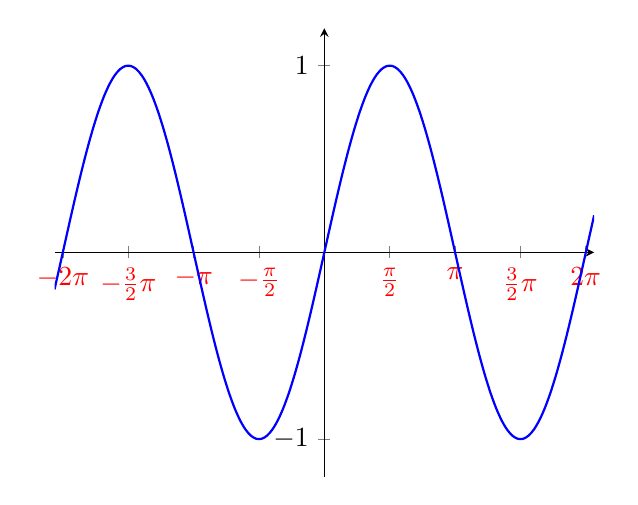
\begin{tikzpicture}
            \begin{axis}[
                    domain=-2*pi-0.2:2*pi+0.2,
                    axis lines=middle,
                    ymin=-1.2,
                    ymax=1.2,
                    ytick={-1,1},
                    xtick={-6.28, -4.71, -3.14,-1.57, 1.57, 3.14, 4.71, 6.28},
                    xticklabels={$-2\pi$, $-\frac{3}{2}\pi$, $-\pi$, $-\frac{\pi}{2}$, $\frac{\pi}{2}$, $\pi$, $\frac{3}{2}\pi$, $2\pi$},
                    xticklabel style={red}
                ]
                \addplot[blue,thick,solid,smooth,samples=100]{sin(deg(x))} 
                ;
            \end{axis}
        \end{tikzpicture}
    \end{figure}

    \begin{figure}[p]
        \centering
        \caption{Wykres $cos\varphi$}
        \label{fig:wykres_cos}
        \vspace{3mm}
        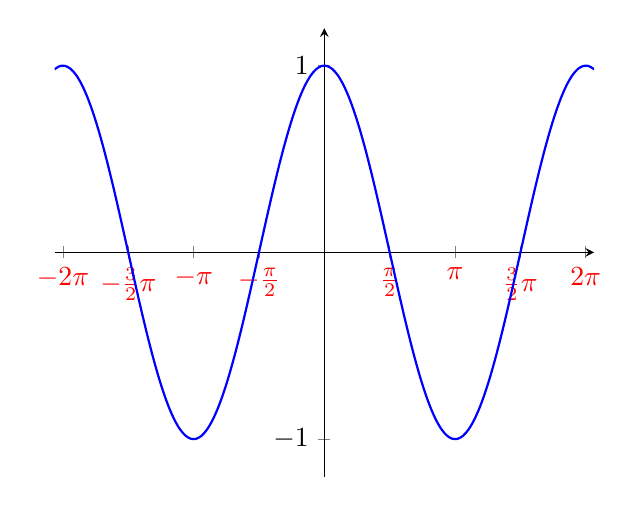
\begin{tikzpicture}
            \begin{axis}[
                    domain=-2*pi-0.2:2*pi+0.2,
                    axis lines=middle,
                    ymin=-1.2,
                    ymax=1.2,
                    ytick={-1,1},
                    xtick={-6.28, -4.71, -3.14,-1.57, 1.57, 3.14, 4.71, 6.28},
                    xticklabels={$-2\pi$, $-\frac{3}{2}\pi$, $-\pi$, $-\frac{\pi}{2}$, $\frac{\pi}{2}$, $\pi$, $\frac{3}{2}\pi$, $2\pi$},
                    xticklabel style={red}
                ]
                \addplot[blue,thick,solid,smooth,samples=100]{cos(deg(x))} 
                ;
            \end{axis}
        \end{tikzpicture}
    \end{figure}

    \begin{figure}[p]
        \centering
        \caption{Wykres $tg\varphi$}
        \label{fig:wykres_tg}
        \vspace{3mm}
        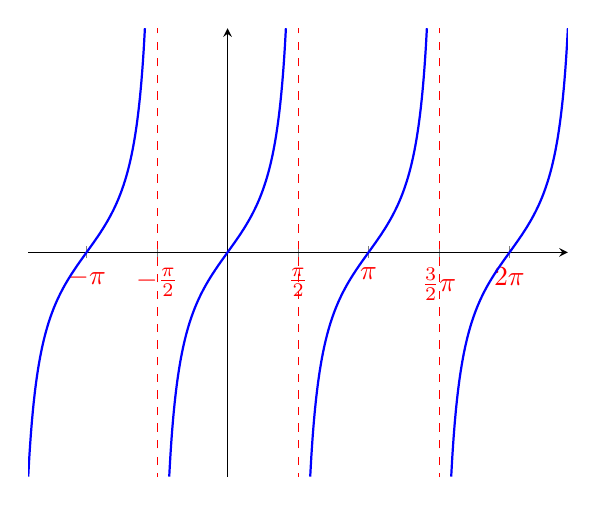
\begin{tikzpicture}
            \begin{axis}[
                    domain=-2*pi-0.2:2*pi+0.2,
                    axis lines=middle,
                    ytick={0},
                    xtick={-6.28, -4.71, -3.14,-1.57, 1.57, 3.14, 4.71, 6.28},
                    xticklabels={$-2\pi$, $-\frac{3}{2}\pi$, $-\pi$, $-\frac{\pi}{2}$, $\frac{\pi}{2}$, $\pi$, $\frac{3}{2}\pi$, $2\pi$},
                    xticklabel style={red}
                ]
                \draw[dashed,red] (-0.5*pi,-100) -- (-0.5*pi,100);
                \draw[dashed,red] (0.5*pi,-100) -- (0.5*pi,100);
                \draw[dashed,red] (1.5*pi,-100) -- (1.5*pi,100);
                \addplot[blue,thick,solid,smooth,samples=100,domain=-1*pi-1.3:-1*pi+1.3]{tan(deg(x))}; 
                \addplot[blue,thick,solid,smooth,samples=100,domain=1*pi-1.3:1*pi+1.3]{tan(deg(x))};
                \addplot[blue,thick,solid,smooth,samples=100,domain=-1.3:1.3]{tan(deg(x))}; 
                \addplot[blue,thick,solid,smooth,samples=100,domain=2*pi-1.3:2*pi+1.3]{tan(deg(x))};
                ;
            \end{axis}
        \end{tikzpicture}
    \end{figure}

    \begin{figure}[p]
        \centering
        \caption{Wykres $ctg\varphi$}
        \label{fig:wykres_ctg}
        \vspace{3mm}
        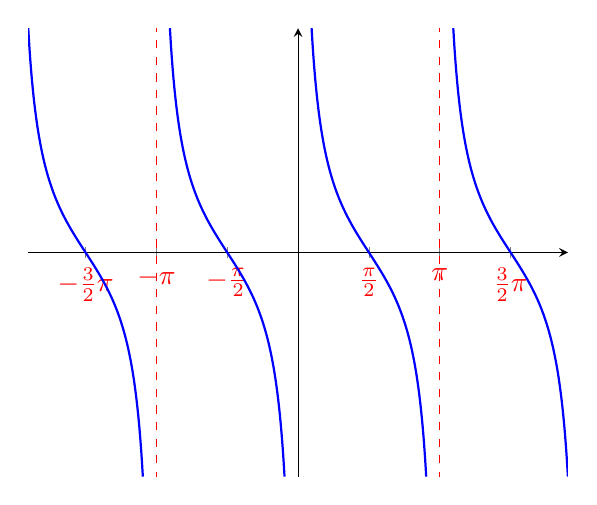
\begin{tikzpicture}
            \begin{axis}[
                    domain=-2*pi-0.2:2*pi+0.2,
                    axis lines=middle,
                    ytick={0},
                    xtick={-6.28, -4.71, -3.14,-1.57, 1.57, 3.14, 4.71, 6.28},
                    xticklabels={$-2\pi$, $-\frac{3}{2}\pi$, $-\pi$, $-\frac{\pi}{2}$, $\frac{\pi}{2}$, $\pi$, $\frac{3}{2}\pi$, $2\pi$},
                    xticklabel style={red}
                ]
                \draw[dashed,red] (-1*pi,-100) -- (-1*pi,100);
                \draw[dashed,red] (pi,-100) -- (pi,100);
                \draw[dashed,red] (2*pi,-100) -- (2*pi,100);
                \addplot[blue,thick,solid,smooth,samples=100,domain=-2*pi+0.3:-1*pi-0.3]{cot(deg(x))};
                \addplot[blue,thick,solid,smooth,samples=100,domain=-1*pi+0.3:-0.3]{cot(deg(x))}; 
                \addplot[blue,thick,solid,smooth,samples=100,domain=0.3:1*pi-0.3]{cot(deg(x))};
                \addplot[blue,thick,solid,smooth,samples=100,domain=pi+0.3:2*pi-0.3]{cot(deg(x))}; 
                ;
            \end{axis}
        \end{tikzpicture}
    \end{figure}

    \begin{table}[htbp]
        \footnotesize
        \centering
        \caption{Wzory redukcyjne funkcji trygonometrycznych}
        \label{tab:wzory_redukcyjne_tryg}
        \vspace{3mm}
        \begin{tabular}{c|c|cc|cc|cc|}
             & I ćwiartka & \multicolumn{2}{|c|}{II ćwiartka} & \multicolumn{2}{|c|}{III ćwiartka} & \multicolumn{2}{|c|}{III ćwiartka}\\
             \midrule
             \multirow{2}{*}{$\varphi$} & $90\degree - \alpha$ & $90\degree+\alpha$ & $180\degree - \alpha$ & $180\degree+\alpha$ & $270\degree - \alpha$ & $270\degree+\alpha$ & $360\degree-\alpha$ \\
             & $\frac{\pi}{2} - \alpha$ & $\frac{\pi}{2} + \alpha$ & $\pi - \alpha$ & $\pi + \alpha$ & $\frac{3}{2}\pi - \alpha$ & $\frac{3}{2}\pi + \alpha$ & $2\pi - \alpha$ \\ 
             \midrule
            $sin \varphi$ & $cos\alpha$ & $cos\alpha$ & $sin\alpha$ & $-sin\alpha$ & $-cos\alpha$ & $-cos\alpha$ & $-sin\alpha$ \\
            $cos \varphi$ & $sin\alpha$ & $-sin\alpha$ & $-cos\alpha$ & $-cos\alpha$ & $-sin\alpha$ & $cos\alpha$ & $sin\alpha$ \\
            $tg \varphi$ & $ctg\alpha$ & $-ctg\alpha$ & $-tg\alpha$ & $tg\alpha$ & $ctg\alpha$ & $-ctg\alpha$ & $-tg\alpha$ \\
            $ctg \varphi$ & $tg\alpha$ & $-tg\alpha$ & $-ctg\alpha$ & $ctg\alpha$ & $tg\alpha$ & $-tg\alpha$ & $-ctg\alpha$ \\
            \bottomrule
        \end{tabular}
    \end{table}

    \begin{table}[h!]
        \centering
        \caption{Wartości funkcji trygonometrycznych ważniejszych kątów}
        \label{tab:wartosci_tryg}
        \vspace{3mm}
        \begin{tabular}{cccccc}
            \multicolumn{2}{c}{$\varphi$} & \multirow{2}{*}{$sin\varphi$} & \multirow{2}{*}{$cos\varphi$} & \multirow{2}{*}{$tg\varphi$} & \multirow{2}{*}{$ctg\varphi$} \\
            deg & rad & & & &\\
            \midrule
            $0\degree$ & 0 & 0 & 1 & 0 & -\\
            $15\degree$ & $\frac{\pi}{12}$ & $\frac{\sqrt{6}-\sqrt{2}}{4}$ & $\frac{\sqrt{6}+\sqrt{2}}{4}$ & $2-\sqrt{3}$ & $2+\sqrt{3}$\\
            $30\degree$ & $\frac{\pi}{6}$ & $\frac{1}{2}$ & $\frac{\sqrt{3}}{2}$ & $\frac{\sqrt{3}}{3}$ & $\sqrt{3}$\\
            $45\degree$ & $\frac{\pi}{4}$ & $\frac{\sqrt{2}}{2}$ & $\frac{\sqrt{2}}{2}$ & $1$ & $1$\\
            $60\degree$ & $\frac{\pi}{3}$ & $\frac{\sqrt{3}}{2}$ & $\frac{1}{2}$ & $\sqrt{3}$ & $\frac{\sqrt{3}}{3}$\\
            $75\degree$ & $\frac{5\pi}{12}$ & $\frac{\sqrt{6}+\sqrt{2}}{4}$ & $\frac{\sqrt{6}-\sqrt{2}}{4}$ & $2+\sqrt{3}$ & $2-\sqrt{3}$\\
            $90\degree$ & $\frac{\pi}{2}$ & 1 & 0 & - & 0\\
            $180\degree$ & $\pi$ & 0 & -1 & 0 & -\\
            $270\degree$ & $\frac{3\pi}{2}$ & -1 & 0 & 1 & 0\\
            $360\degree$ & $2\pi$ & 0 & 1 & 0 & -\\
            \bottomrule
        \end{tabular}
    \end{table}

\renewcommand{\arraystretch}{1}

    \printindex
\end{document}
